\documentclass[text05.tex]{subfiles}
\begin{document}
\chapter{Raspberry Piをリモコンにしてみよう}
\section{はじめに}
\subsection{この章で学ぶこと}

この章では、以下のことを学びます。

\begin{itemize}
  \item 入力\ruby{装置}{そう|ち}と出力\ruby{装置}{そう|ち}の\ruby{違}{ちが}い
  \item デジタル信号とアナログ信号の\ruby{違}{ちが}い
  \item FaBoを使って、センサーや出力\ruby{装置}{そう|ち}をRaspberry Piに
        \ruby{接続}{せつ|ぞく}する方法
  \item センサーから受け取った\ruby{値}{あたい}をプログラムで利用する方法
  \item 赤外線リモコンの信号を記録して送信する方法
\end{itemize}

「入力\ruby{装置}{そう|ち}と出力\ruby{装置}{そう|ち}」では、
ボタンやセンサーからRaspberry Piへ\ruby{情報}{じょう|ほう}を送る方法と、
LEDや\ruby{振動子}{しん|どう|し}などをRaspberry Piから動かす方法を学びます。

「デジタル信号とアナログ信号」では、
0と1で表す信号と、0から1023までの数値で表す信号の
\ruby{違}{ちが}いを学びます。

「FaBoの\ruby{操作}{そう|さ}」では、
いろいろなセンサーや出力\ruby{装置}{そう|ち}をRaspberry Piにつなぎ、
データを入力したり、プログラムから\ruby{装置}{そう|ち}を動かしたりする
方法を学びます。

「赤外線リモコンの信号」では、
赤外線とは何かを学び、リモコンの信号を読み取って記録し、
Raspberry Piから同じ信号を送信する方法を学びます。

\subsection{教材を自分のフォルダに置こう}
まずは、今回利用する教材をコピーしましょう。
教材は、ディレクトリ \nobreak/usr/local/share/ome/05 に入っています。このディレクトリをホームディレクトリにコピーしましょう。

\newpage
\section{センサーの\ruby{基本}{き|ほん}}
\subsection{センサーってなんだろう？}
センサーは身の回りの世界の\ruby{情報}{じょう|ほう}を調べ、コンピュータに伝えるための装置です。明るさ、温度、\ruby{湿度}{しつ|ど}を調べることができるセンサーボードは第3回の\ruby{授業}{じゅ|ぎょう}で\ruby{扱}{あつか}いました。しかし、センサーはたくさんの種類があり、出来ることももっとたくさんあります。まず、スマートフォンで使われているセンサーを見てみましょう。
\begin{figure}[htb]
\begin{center}
    \includesvg[width=1.0\linewidth]{../../asset/image/smartphone_sensors.svg}
    \caption{スマートフォンに使われているセンサー}
    \label{fig1}
\end{center}
\end{figure}
\begin{table}[htb]
  \caption{スマートフォンに使われているセンサーの種類とできること}
  \label{table-sensors}
  \centering
  \begin{widerrows}[1.3] 
    \begin{tabular}{|l|l|} \hline
      \multicolumn{1}{|c|}{センサーの種類} & \multicolumn{1}{c|}{できること} \\ \hline\hline
      GPSセンサー & 自分のいる位置が分かるようになる \\
      \ruby{磁気}{じ|き}センサー & \ruby{磁力}{じ|りょく}を検知して方角を示す \\
      \ruby{加速度}{か|そく|ど}センサー & スマートフォンの向きを調べる \\
      ジャイロセンサー & スマートフォンの回転スピードを調べる \\
      \ruby{環境光}{かん|きょう|こう}センサー & 周りの明るさを調べる \\
      \ruby{近接}{きん|せつ}センサー & 近づいてくるものを調べる \\
      \ruby{指紋}{し|もん}センサー & \ruby{指紋}{し|もん}パターンを調べる \\
      タッチセンサー & スマホのどこをタップしたかを調べる \\\hline
    \end{tabular}
  \end{widerrows} 
\end{table}

このように、機械では多くのセンサーが使われています。今日の授業ではセンサーをいくつか扱います。どのセンサーが何に使えそうか、何に使われていそうかを考えながら使ってみましょう。

\subsection{アナログ信号とデジタル信号}
センサーが出力するデータは大きく分けて２種類あり、デジタル信号とアナログ信号と\ruby{呼}{よ}ばれる信号のどちらを使うかで分けられています。２つの信号には以下の図のような\ruby{違}{ちが}いがあります。
\begin{figure}[htbp]
  \begin{minipage}[b]{0.5\linewidth}
    \centering
    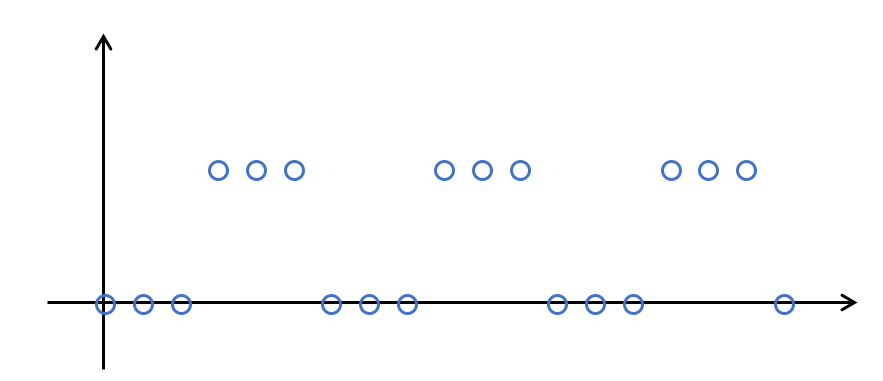
\includegraphics[keepaspectratio, scale=0.5]{../../asset/image/text05-img002.png}
    \caption{デジタル信号の例}
    \label{fig2}
  \end{minipage}
  \begin{minipage}[b]{0.5\linewidth}
    \centering
    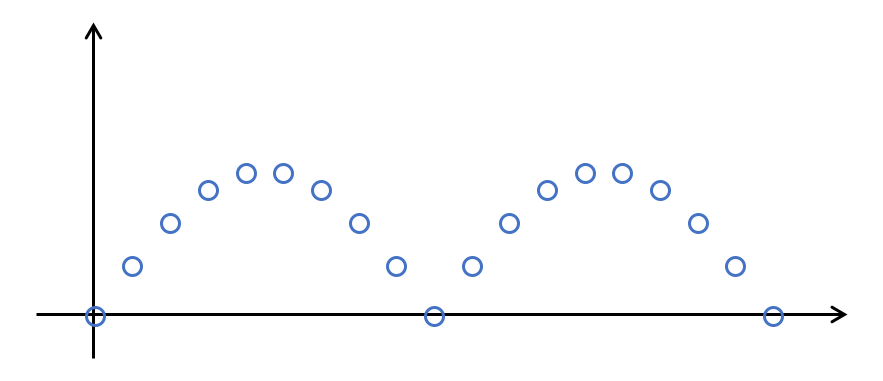
\includegraphics[keepaspectratio, scale=0.5]{../../asset/image/text05-img003.png}
    \caption{アナログ信号の例}
    \label{fig3}
  \end{minipage}
\end{figure}

図\ref{fig2}と図\ref{fig3}はコンピュータで使われている信号をグラフにしたものです。授業で使用するセンサーのデジタル信号は、図\ref{fig2}と図\ref{fig3}のように２種類の\ruby{値}{あたい}を表すことができます。２種類の値は０か１です。一方授業で使用するアナログ信号は、\ref{fig3}のように中間の値を表すことができます。この値は0〜1023の数字で\ruby{表現}{ひょう|げん}されます。

デジタル信号はボタンが\ruby{押}{お}されたか押されていないか、明かりがついたか消えたかなどのふた通りのものを表すときに使われ、アナログ信号は主に明るさや距離などの数を表すときに使われます。

\begin{tcolorbox}[title=\useOmetoi]
  \begin{enumerate}
  \addquiz{センサーとはなんだろう。説明してみましょう。}
  \addquiz{スマートフォンで使われているセンサーを3つ書いてみましょう。}
  \addquiz{アナログ信号、デジタル信号の違いを書いてみましょう。}
\end{enumerate}
\end{tcolorbox}
\end{document}
